\chapter{Deseño de software}
O longo deste capítulo detállase a arquitectura do sistema a desenvolver. Mostrase primeiro a arquitectura xeral e a súa interacción con sistemas externos e posteriormente detallase máis polo miúdo a estrutura das distintas compoñentes do sistema.

\section{Arquitectura do sistema}
Dende a definición dos obxectivos do proxecto se identifican dúas partes diferenciadas dentro do sistema a desenvolver. Por un lado a comunicación co servidor SOS, para a obtención das súas capacidades e dos datos de observacións, e por outro a visualización e explotación das observacións descargadas.

Para unha mellor comprensión divídese o subsistema encargado da comunicación co SOS en dous, quedando o sistema global dividido en tres compoñentes:
\begin{description}
\item[SOS Client:] Responsable da interacción co usuario para a comunicación co servidor SOS.
\item[SOS:] Responsable da comunicación co servidor SOS e de interpretar e almacenar a información do servizo.
\item[SOS Plot:] Responsable da visualización das observacións.
\end{description}

Na figura \ref{fig:diaComponentes} represéntanse as tres compoñentes descritas, acompañadas polas compoñentes externas coas que cooperan.

\begin{figure}[hbtp]
 \centering
 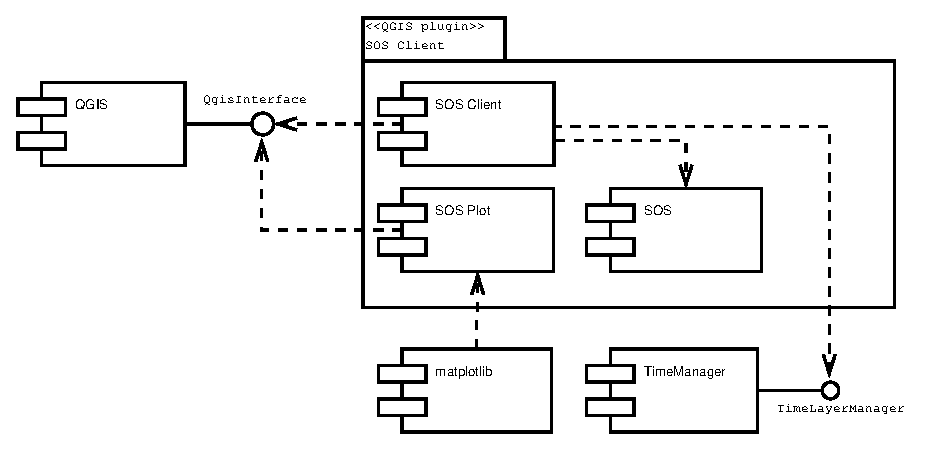
\includegraphics[width=\textwidth]{images/componentes.eps}
 \caption{Diagrama de compoñentes}
 \label{fig:diaComponentes}
\end{figure}

\subsection{Patrón de arquitectura}
O uso dun patrón de arquitectura axeitado para o sistema a desenvolver facilita os procesos de implementación e probas, ó proporcionar un esquema de organización estrutural dividindo o sistema en partes segundo a súa responsabilidade.

Os patróns de arquitectura máis amplamente utilizados no desenvolvemento de aplicacións con interface gráfica son o MVC (Model-View-Controller) e os seus derivados. O obxectivo principal destes patróns é separar o modelo de datos, a súa visualización e a lóxica de negocio facilitando de xeito moi significativo o mantemento e evolución das aplicacións.

TODO: Describir MVVM, que se usa por escasa lógica de negocio, rigidez librerías gráficas

%O patrón MVP (Model-View-Controller), que se amosa na figura \ref{fig:diaMVP}, é un patrón derivado do MVC, con algunhas diferencias\cite{MVPvsMVC} que fan que sexa o patrón elixido para aplicar neste proxecto. Estas diferencias son, de xeito resumido:
%\begin{itemize}
%\item No MVP vista e modelo son completamente independentes.
%\item A vista é tan sinxela que non necesita ser testada.
%\item O modelo MVP está enfocado o desenvolvemento guiado por probas ou TDD\cite{TDDPython} (do inglés Test Driven Development).
%\end{itemize}
%
%\begin{figure}[hbtp]
% \centering
% \includegraphics[scale=1]{images/MVP.png}
% \caption{Diagrama do patrón de deseño MVP}
% \label{fig:diaMVP}
%\end{figure}

\section{Diagramas de secuencia}
Para describir o comportamento do sistema desde un punto de vista dinámico empréganse os diagramas de secuencia, nos que se describe a interacción entre as distintas compoñentes do sistema para cumprir cada caso de uso definido.

No diagrama \ref{fig:diaSeq1-2} inclúense os caso de uso \ref{uc:CU.01} e \ref{uc:CU.02}, xa que o \ref{uc:CU.02} estende ó \ref{uc:CU.01}, polo que é máis claro representalos xuntos.
\begin{figure}
 \centering
 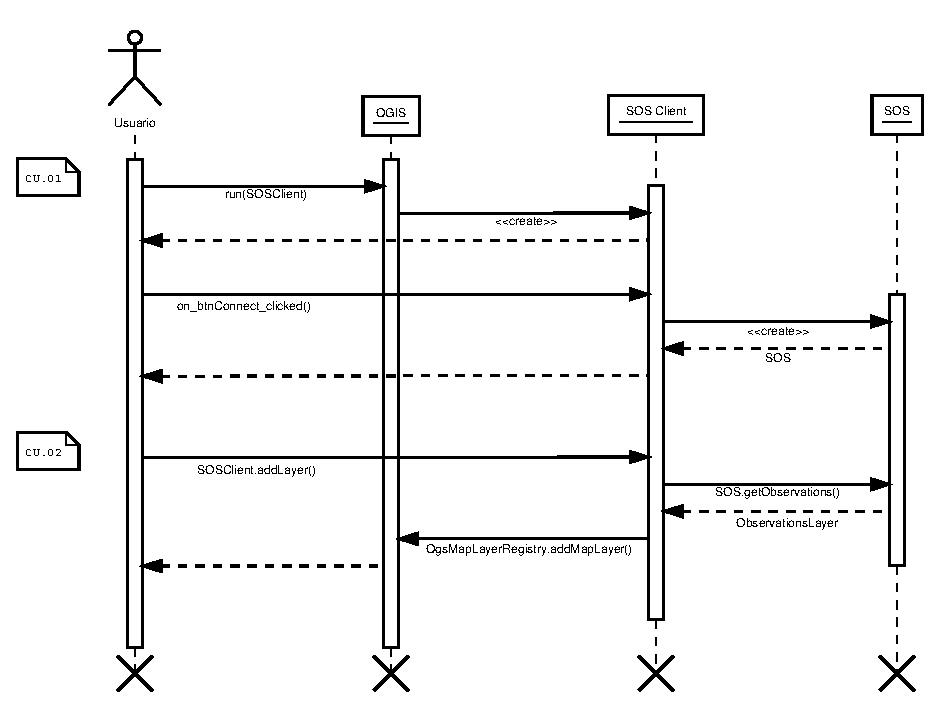
\includegraphics[width=\textwidth]{images/seq1-2.eps}
 \caption{Diagrama de secuencia para os casos de uso \ref{uc:CU.01} e \ref{uc:CU.02}}
 \label{fig:diaSeq1-2}
\end{figure}

O diagrama \ref{fig:diaSeq3} representa o comportamento para o caso de uso \ref{uc:CU.03}.
\begin{figure}
 \centering
 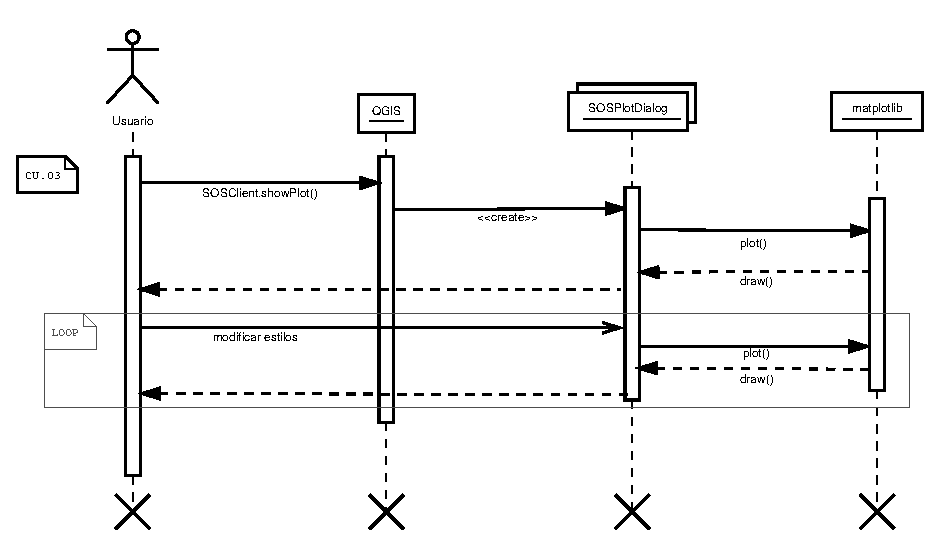
\includegraphics[width=\textwidth]{images/seq3.eps}
 \caption{Diagrama de secuencia para o caso de uso \ref{uc:CU.03}}
 \label{fig:diaSeq3}
\end{figure}

Para o caso de uso \ref{uc:CU.04} existe o \emph{plugin} \emph{TimeManager} para QGIS, que proporciona a funcionalidade necesaria, polo que o que representa o diagrama \ref{fig:diaSeq4} é o procedemento para que a capa xerada coas observacións sexa controlada polo \emph{TimeManager}.
\begin{figure}
 \centering
 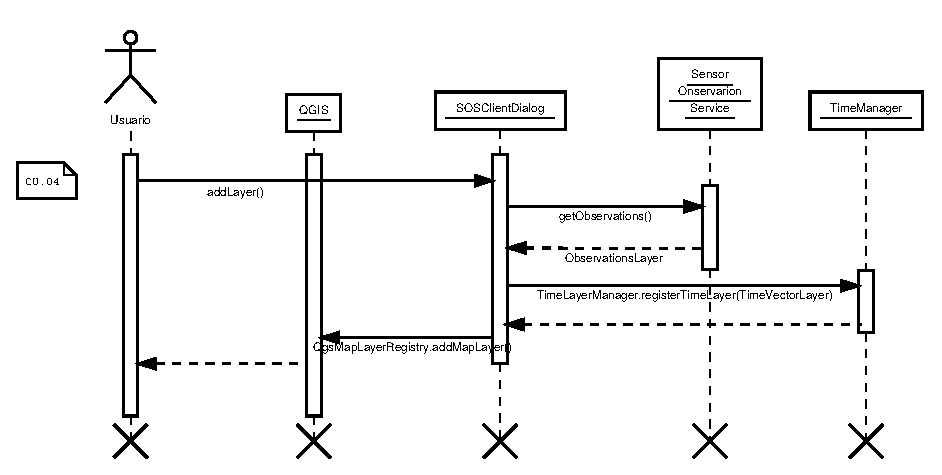
\includegraphics[width=\textwidth]{images/seq4.eps}
 \caption{Diagrama de secuencia para o caso de uso \ref{uc:CU.04}}
 \label{fig:diaSeq4}
\end{figure}

\section{Diagramas de clases}
A continuación descríbese máis en detalle cada unha das compoñentes do sistema a desenvolver, representando as clases máis relevantes de cada unha. Nos diagramas de clase so se mostran os atributos e métodos máis relevantes para entender o a función de cada unha delas.

No diagrama \ref{fig:diaClassSOSClient} móstrase a clase SOSClient, que actúa como punto de entrada ó \emph{plugin}, e a clase SOSClientDialog que é a clase principal da compoñente SOSClient, pois é a que actúa como \emph{ViewModel} para permitir ó usuario manipular co \emph{Model} gardado no seu atributo \emph{service}. A clase \emph{QgsMapToolCaptureSpatialOperand} é a encargada de interacionar co mapa para seleccionar sobre el as zonas a usar como filtro espacial. E por último, tamén se mostra a clase SOSPlotDialog que non forma parte deste compoñente, pero representase para mostrar que depende tamén da clase SOSClient.

\begin{figure}
 \centering
 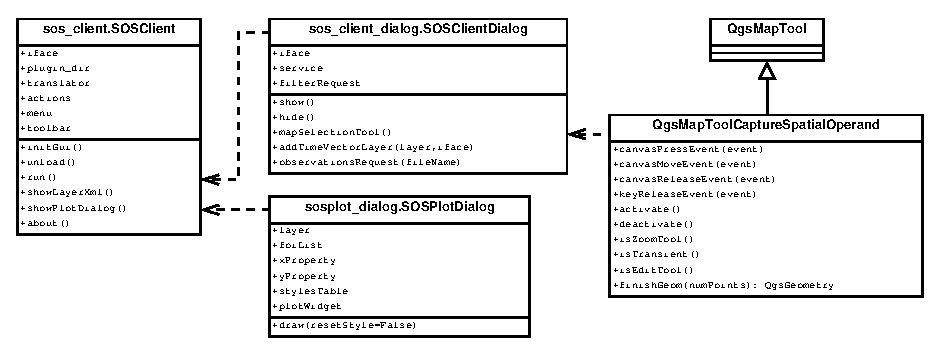
\includegraphics[width=\textwidth]{images/clases_sos_client.eps}
 \caption{Diagrama de clases da compoñente SOS Client}
 \label{fig:diaClassSOSClient}
\end{figure}

No diagrama \ref{fig:diaClassSOS} móstranse as clases encargadas de almacenar a e procesar a información do servizo SOS. A clase SensorObservationService é a que representa o servizo e a que actúa como \emph{Model} para a clase \emph{SOSClientDialog} (diagrama \ref{fig:diaClassSOSClient}). As outras clases máis relevantes desta da compoñente SOS son a ObservationsLayer e SOSProvider, pois son as encaradas de transformar as observacións en XML a unha capa vectorial (QgsVectorLayer).
As clases encadradas no fondo gris son as adicadas ó procesamento do XML.
\begin{sidewaysfigure}
 \centering
 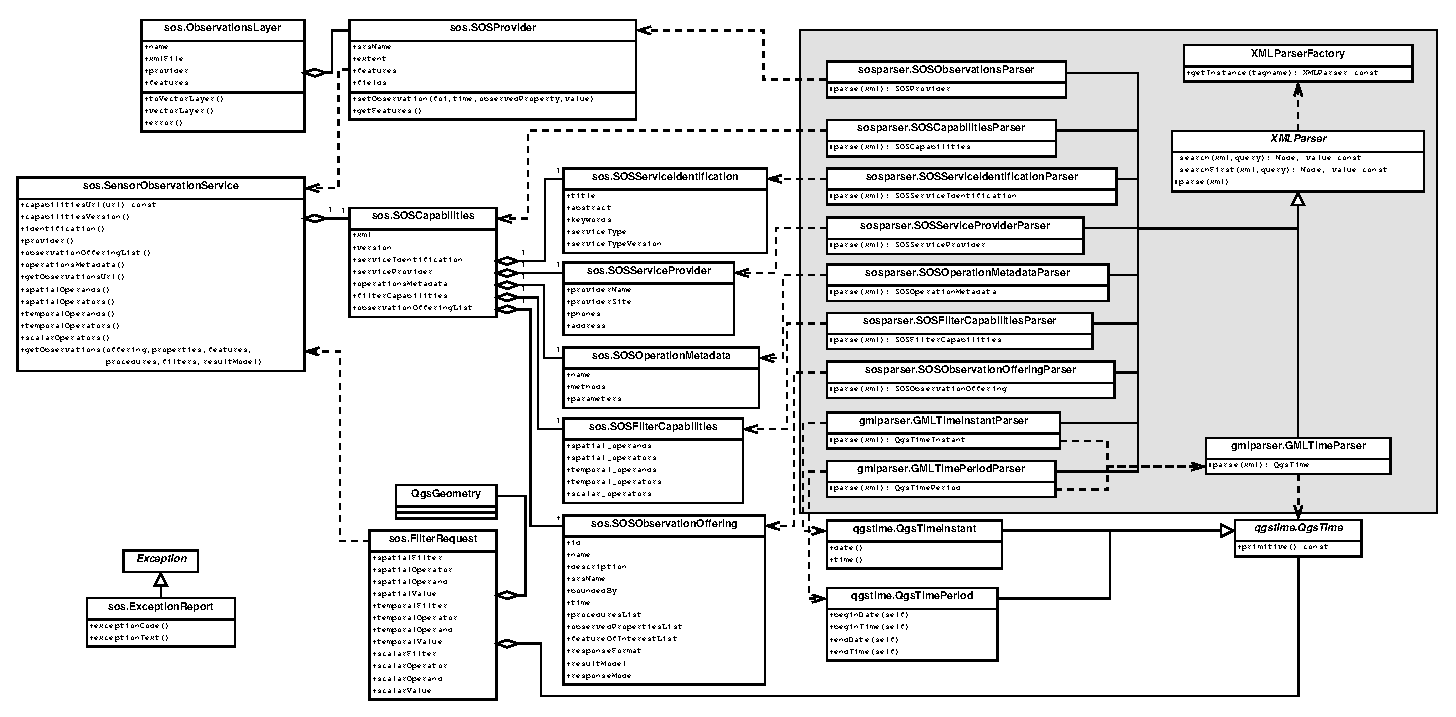
\includegraphics[width=\textwidth]{images/clases_sos.eps}
 \caption{Diagrama de clases da compoñente SOS}
 \label{fig:diaClassSOS}
\end{sidewaysfigure}

No diagrama \ref{fig:diaClassSOSPlot} móstranse as clases encargadas de visualizar os gráficos en dúas dimensións. A clase SOSPlotDialog actúa como \emph{ViewModel} e como \emph{Model} actúa a propia capa do QGIS (QgsVectorLayer), polo que non se presenta.

\begin{figure}
 \centering
 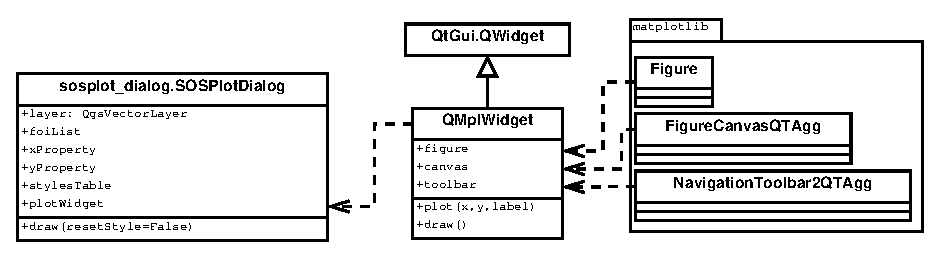
\includegraphics[width=\textwidth]{images/clases_sos_plot.eps}
 \caption{Diagrama de clases da compoñente SOS Plot}
 \label{fig:diaClassSOSPlot}
\end{figure}

Non se representan en ningún diagrama as clases correspondentes as \emph{View} xa que estas son xeradas automaticamente a partir da súa definición XML pola clase WidgetFactory implementada a tal efecto.